\chapter{Methodology}

You are expected to be methodical in your work, so that it could and can be
reproduced and replicated by others to verify your results.
If you are clear in your methodology, you will have a better chance of someone
building on your work \cite{villaneuva18}.
That will lead to more people being interested in what you have done, and will
give you a higher profile.
Remember that undergraduate students will sometimes do projects based on
academic research, so it's a good idea to be explicit enough that they can
easily replicate your results.

It is important that you demonstrate that you were methodical from the start.
While it is tempting to play around with various algorithms or techniques
before you really sit down to work.
If you take five minutes beforehand to think through what you are about to do
and write it down, you will quickly build up a portfolio of writing and results
that can go into your thesis.
There is often very little pracitcal difference between being methodical and
playing around -- it's largely in your attitude while you are doing the work.

Note that \LaTeX has a lot of nice functionality for creating various types of
plots and diagrams.
Check out the nice graphs in Figure \ref{tikz:graphs}.

\lipsum[26]

\begin{figure}[ht]
  \centering
  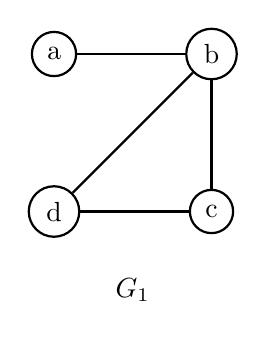
\begin{tikzpicture}
    \begin{scope}[every node/.style={circle,thick,draw}]
      \node (a) at (0,2) {a};
      \node (b) at (2,2) {b};
      \node (c) at (2,0) {c};
      \node (d) at (0,0) {d};
    \end{scope}
    \begin{scope}[every edge/.style={draw=black,thick}]
      \path (a) edge (b);
      \path (b) edge (c);
      \path (b) edge (d);
      \path (c) edge (d);
    \end{scope}
    \node () at (1,-1) {$G_1$};
  \end{tikzpicture}
  \hspace{1.5cm}
  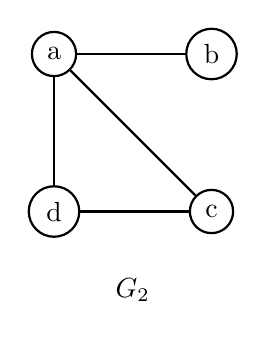
\begin{tikzpicture}
    \begin{scope}[every node/.style={circle,thick,draw}]
      \node (1) at (0,2) {a};
      \node (2) at (2,2) {b};
      \node (3) at (2,0) {c};
      \node (4) at (0,0) {d};
    \end{scope}
    \begin{scope}[every edge/.style={draw=black,thick}]
      \path (1) edge (2);
      \path (1) edge (3);
      \path (1) edge (4);
      \path (3) edge (4);
    \end{scope}
    \node () at (1,-1) {$G_2$};
  \end{tikzpicture}
  \caption{Nice pictures}
  \label{tikz:graphs}
\end{figure}

\section{Vector Spaces}

A \textbf{vector space} $V$ over a field $\mathbb{F}$ is a set equipped with two operations:

\begin{itemize}
    \item Vector addition: $+: V \times V \rightarrow V$, denoted as $(\mathbf{v}, \mathbf{w}) \mapsto \mathbf{v} + \mathbf{w}$.
    \item Scalar multiplication: $\cdot: \mathbb{F} \times V \rightarrow V$, denoted as $(\lambda, \mathbf{v}) \mapsto \lambda \mathbf{v}$.
\end{itemize}
These operations must satisfy the following properties for all $\mathbf{u}, \mathbf{v}, \mathbf{w} \in V$ and $\lambda, \mu \in \mathbb{F}$:

\begin{enumerate}
    \item \textbf{Addition is commutative}: $\mathbf{u} + \mathbf{v} = \mathbf{v} + \mathbf{u}$.
    \item \textbf{Addition is associative}: $(\mathbf{u} + \mathbf{v}) + \mathbf{w} = \mathbf{u} + (\mathbf{v} + \mathbf{w})$.
    \item \textbf{Additive identity}: There exists a vector $\mathbf{0} \in V$ such that $\mathbf{v} + \mathbf{0} = \mathbf{v}$ for all $\mathbf{v} \in V$.
    \item \textbf{Additive inverse}: For every vector $\mathbf{v} \in V$, there exists a vector $-\mathbf{v} \in V$ such that $\mathbf{v} + (-\mathbf{v}) = \mathbf{0}$.
    \item \textbf{Scalar multiplication is distributive over vector addition}: $\lambda (\mathbf{v} + \mathbf{w}) = \lambda \mathbf{v} + \lambda \mathbf{w}$.
    \item \textbf{Scalar multiplication is distributive over scalar addition}: $(\lambda + \mu) \mathbf{v} = \lambda \mathbf{v} + \mu \mathbf{v}$.
    \item \textbf{Scalar multiplication is associative}: $(\lambda \mu) \mathbf{v} = \lambda (\mu \mathbf{v})$.
    \item \textbf{Scalar multiplication identity}: $1 \cdot \mathbf{v} = \mathbf{v}$, where $1$ is the multiplicative identity in $\mathbb{F}$.
\end{enumerate}


\section{Dirac Notation}
Dirac notation, also known as bra-ket notation, is a powerful and concise mathematical notation used extensively in quantum mechanics.
It was introduced by the physicist Paul Dirac and provides a convenient way to represent vectors, linear operators, and inner products in quantum mechanics.
Here's a breakdown of the components of Dirac notation:

\begin{description}
  \item[Ket notation $\ket{\psi}$:]
  A ket is represented by a column vector enclosed within vertical bars.
  It represents a state vector in a complex vector space.
  For example, $\ket{\psi}$ could represent the state of a quantum system.

  \item[Bra notation $\bra{\psi}$:]
  A bra is represented by a row vector enclosed within angular brackets.
  It represents the complex conjugate transpose of a ket vector.
  If $\ket{\psi}$ represents a state vector, then $\ket{\psi}$ represents the corresponding bra vector.

  \item[Inner product ($\braket{\psi \mid \psi}$):]
  The inner product of two vectors is represented by placing a bra vector on the left and a ket vector on the right, enclosed within angular brackets.
  It yields a complex number and is a measure of the "overlap" between the two vectors.
  In quantum mechanics, the inner product is used to calculate probabilities and to determine the expectation values of observables.

  \item[Outer product ($\ket{\psi}\bra{\phi}$):]
  The outer product of two vectors is represented by placing a ket vector on the left and a bra vector on the right.
  It results in a linear operator known as a ket-bra or dyad, which maps one vector to another.
  In quantum mechanics, outer products are used to represent quantum operators.

  \item[Operators ($A\ket{\psi}$):]
  If $A$ is a linear operator, its action on a ket vector $\ket{\psi}$ is represented by placing the operator to the left of the ket vector.
  This notation shows the result of applying the operator to the state vector.
\end{description}
Dirac notation offers several advantages:
\begin{description}
    \item[Clarity and Conciseness:]
    It provides a concise representation of complex mathematical objects, making expressions and calculations easier to write and understand.
    \item[Flexibility:]
    It can be easily extended to represent complex operations and concepts in quantum mechanics, such as composite systems, entanglement, and measurement.
    \item[Computational Efficiency:]
    Dirac notation simplifies many calculations in quantum mechanics, such as computing inner products, expectation values, and transition probabilities.
\end{description}
Overall, Dirac notation is a fundamental tool in quantum mechanics, enabling physicists to express and manipulate quantum states and operations in a clear and efficient manner.
